\section{Results}

\subsection{Nested Dependencies in Neural Language Models}

\subsubsection{Replication of previous results in Italian}
\paragraph{Ablation results}
\paragraph{Dynamics of the number unit} in nounpp
\begin{figure*}
    \centering
    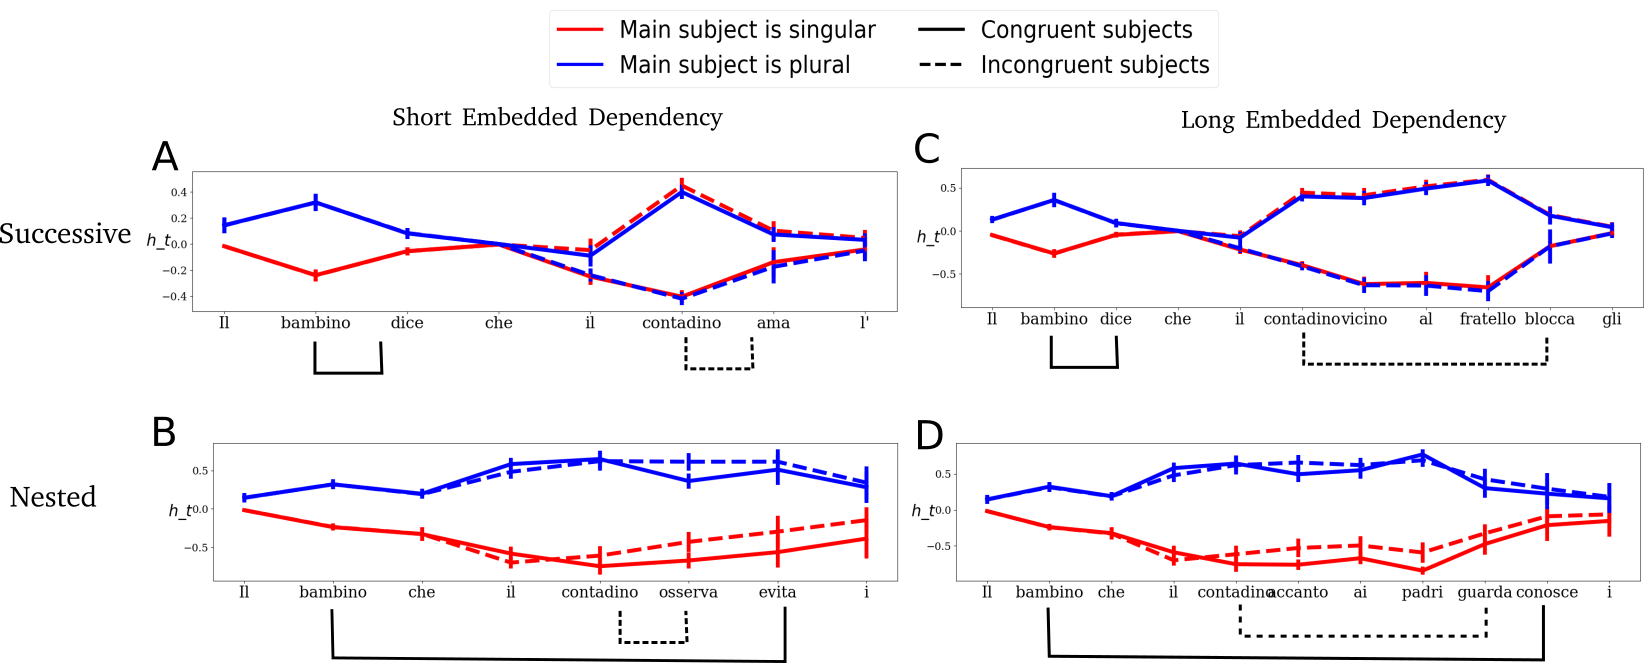
\includegraphics[width=\textwidth]{figures/model_activations.png}
    \caption{\textbf{Dynamics of the hidden activation of the number unit during the processing of two subject-verb dependencies.} Number-unit activity is presented for the four structures in the design: SC-short (panel A), SC-long (B), objRC-short (C) and objRC-long (D). For each structure, results are presented for the four conditions, corresponding to whether the main subject of the sentence is singular (red curves) or plural (blue), and to whether the main and embedded subjects have the same grammatical number (congruent; continuous lines) or not (incongruent; dashed lines).}
    \label{fig:my_label}
\end{figure*}



\subsubsection{The Processing of Nested Dependencies}


\begin{figure*}[h]
    \centering
    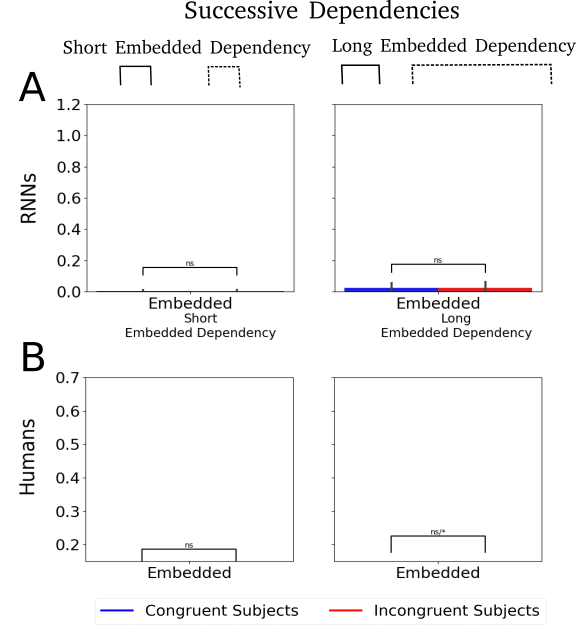
\includegraphics[width=10cm]{figures/error_rates_successive.png}
    \caption{\textbf{Error rates on the SC-short and SC-long structures:} collected from NLMs (panel A) and human subjects (B). Blue and red bars correspond to whether the main and embedded subjects agree on number (congruent subjects) or not (incongruent), respectively). Error bars represent standard error of the mean across all trials. ns - non significant.}
    \label{fig:my_label}
\end{figure*}


\begin{figure*}[h]
    \centering
    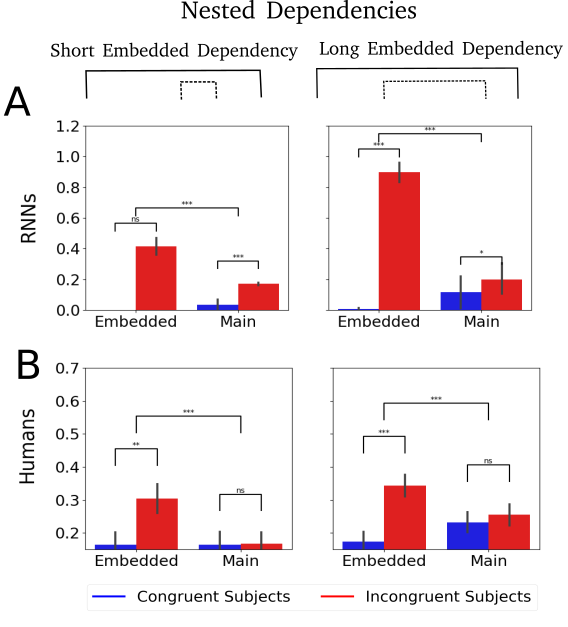
\includegraphics[width=10cm]{figures/error_rates_nested.png}
    \caption{\textbf{Error rates on the objRC-short and objRC-long structures:} collected from NLMs (panel A) and humans subjects (panel B). Blue and red bars correspond to whether the main and embedded subjects agree on number (congruent subjects) or not (incongruent), respectively. Error bars represent standard error of the mean across all trials. ns - non significant.}
    \label{fig:my_label}
\end{figure*}

% \lipsum[1]

\begin{table}[h]
\tiny
\centering
\parbox{.4\linewidth}{
\centering
    \begin{tabular}{ |P{3cm}|P{1.3cm}|P{1.3cm}|  }
    \hline
    \rowcolor{cyan}
    \multicolumn{3}{|c|}{\textbf{Short-Successive}} \\
    \hline
    \rowcolor{cyan}
    \textbf{Effect} & \textbf{Humans} & \textbf{RNNs} \\
    \Xhline{3\arrayrulewidth}
    \rowcolor{green}
    \textbf{Subject Congruence (Embedded verb)} & X & X \\
    \hline
    
    \end{tabular}
}
\hfill
\parbox{.4\linewidth}{
\centering
    \begin{tabular}{ |P{3cm}|P{1.3cm}|P{1.3cm}|  }
    \hline
    \rowcolor{cyan}
    \multicolumn{3}{|c|}{\textbf{Long-Successive}} \\
    \hline
    \rowcolor{cyan}
    \textbf{Effect} & \textbf{Humans} & \textbf{RNNs} \\
    \Xhline{3\arrayrulewidth}
    \rowcolor{green}
    \textbf{Subject Congruence (Embedded verb)} & X & X \\
    \hline
    
    \end{tabular}
}

\vspace{25pt}

\parbox{.4\linewidth}{
\centering
    \begin{tabular}{ |P{3cm}|P{1.3cm}|P{1.3cm}|  }
    \hline
    \rowcolor{cyan}
    \multicolumn{3}{|c|}{\textbf{Short-Nested}} \\
    \hline
    \rowcolor{cyan}
    \textbf{Effect} & \textbf{Humans} & \textbf{RNNs} \\
    \Xhline{3\arrayrulewidth}
    \rowcolor{magenta}
    \textbf{Subject Congruence (Main verb)} & X &  V\\
    \Xhline{3\arrayrulewidth}
    \rowcolor{green}
    \textbf{Subject Congruence (Embedded verb)} & V &  V\\
    \hline
    \rowcolor{green}
    \textbf{Interaction: Subject-Congruence Verb-Position} & V &  V\\
    \hline
    
    \end{tabular}
}
\hfill
\parbox{.4\linewidth}{
\centering
    \begin{tabular}{ |P{3cm}|P{1.3cm}|P{1.3cm}|  }
    \hline
    \rowcolor{cyan}
    \multicolumn{3}{|c|}{\textbf{Long-Nested}} \\
    \hline
    \rowcolor{cyan}
    \textbf{Effect} & \textbf{Humans} & \textbf{RNNs} \\
    \Xhline{3\arrayrulewidth}
    \rowcolor{magenta}
    \textbf{Subject Congruence (Main verb)} & X &  V\\
    \Xhline{3\arrayrulewidth}
    \rowcolor{green}
    \textbf{Subject Congruence (Embedded verb)} & V &  V\\
    \hline
    \rowcolor{green}
    \textbf{Interaction: Subject-Congruence Verb-Position} & V &  V\\
    \hline
    
    \end{tabular}
}
\caption{A summary of all effects  humans and RNNs.}
\label{tbl:comparison}
\end{table}
